\documentclass[../informe_krapp.tex]{subfiles}
\begin{document}
\section{Protocolos de comunicacion}

\subsection{El protocolo de comunicación SPI}
\begin{wrapfigure}{r}{0in}
	\centering
	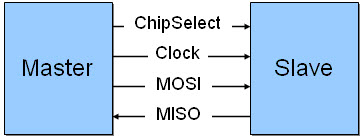
\includegraphics[width= 1.5in, keepaspectratio]{spi-1.jpg}
\end{wrapfigure}

El protocolo Serial Peripheral Interface es un protocolo de comunicación creado por
Motorola, anunciado en el año 1979.
El mismo se divide en 4 lineas de comunicación, cada una con una función específica
(por favor, ver figura \ref{spi-single-slave}) con:

\begin{itemize}
	\item Una señal de clock llamada SCLK, enviada desde el bus master a todos los slaves.
	      Todas las señales del protocolo van as er sínconas a esta señal de clock
	\item Una señal de selección de slave llamada SSn, usada para seleccionar con
	      que slave se esta comunicando el master
	\item Una linea de datos desde master hacia slave, llamada MOSI (Master Out Slave In)
	\item Una linea de datos desde slave hacia master, llamada MISO (Master In Slave OUT)
\end{itemize}

\begin{figure}[H]
	\centering
	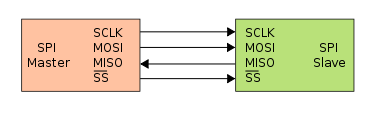
\includegraphics[width=0.5\textwidth]{spi-single-slave.png}
	\caption{SPI master conectado a un único slave.}
	\label{spi-single-slave}
\end{figure}

\begin{figure}[H]
	\centering
	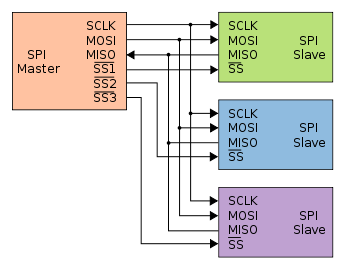
\includegraphics[width=0.5\textwidth]{spi-multiple-slaves.png}
	\caption{SPI master conectado a múltiples slaves.}
	\label{spi-multiple-slaves}
\end{figure}

\clearpage

SPI es un protoclo de comunicación single-master, esto significa que un dispositivo
central (normalmente un microcontrolador) es el encargado de iniciar todas
las comunicaciónes con los slaves.

Cuando el master SPI desea enviar o recibir información de un slave, selecciona el
slave seteando en LOW la linea SS correspondiente, y activa la señal de clock a una
frecuencia usable por el master y el slave.
A partir de ese momento, el master envía la información por el canal MOSI mientras lee
la información que hay en el canal MISO

\begin{figure}[H]
	\centering
	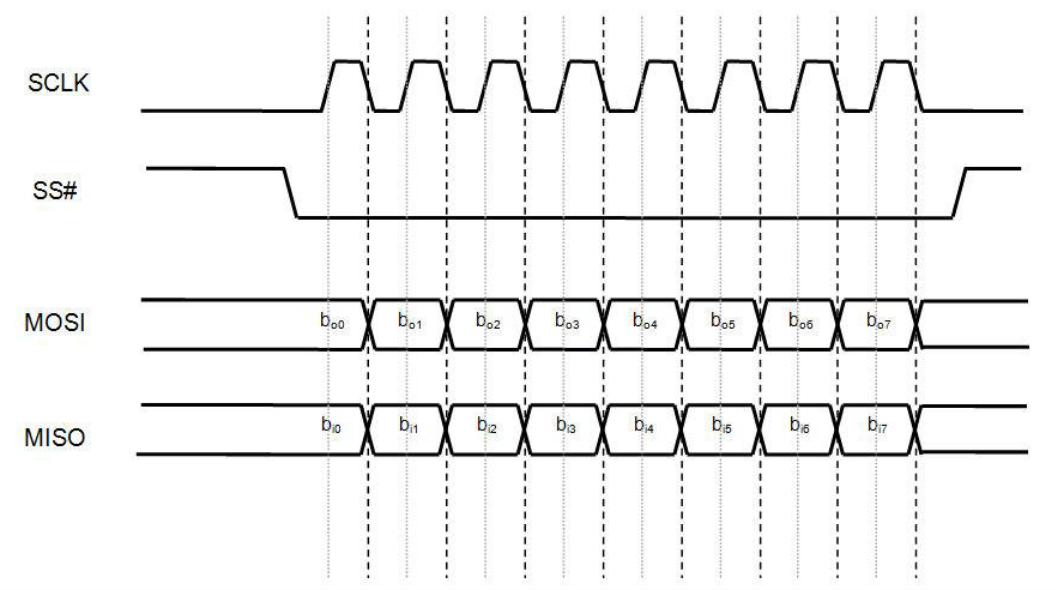
\includegraphics[width=0.7\textwidth]{spi-timing.png}
	\caption{El timing de una comunicación SPI. En este ejemplo,
		La transmisión de datos por los canales MOSI y MISO es ejecutada por
		cada flanco descendente en la señal de clock en SCLK. En cambio,
		la lectura de datos es ejecutada por cada flanco ascendente.
		Esto se puede cambiar modificando el SPI mode }
	\label{spi-timing}
\end{figure}

Como se menciona en la figura \ref{spi-timing}, hay 4 modos SPI, que van del 0 al 3.
Los modos SPI definen en que flanco se activa la linea MOSI, MISO, y el estado (LOW o HIGH)
de inactividad (idle) del canal SCLK.
Cada modo esta definido por un par de parámetros llamados clock polarity
(polaridad de clock) (CPOL), y clock phase (fase de clock) (CPHA)

\begin{figure}[H]
	\centering
	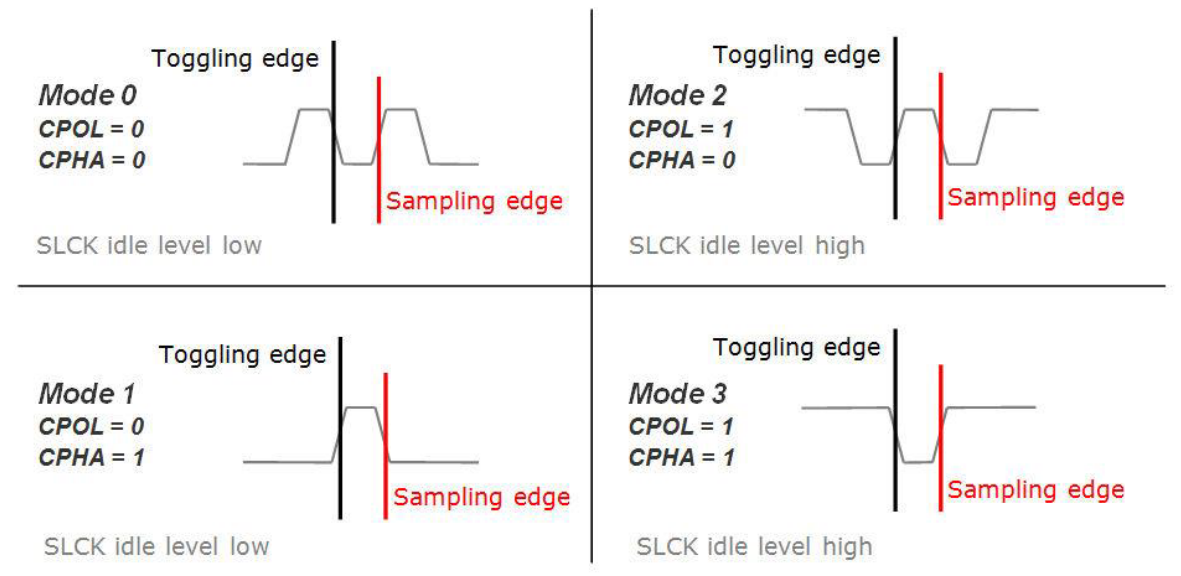
\includegraphics[width=0.7\textwidth]{spi-modes.png}
	\caption{Los modos SPI son definidos con los parámetros CPOL (clock polarity) y CPHA
		(clock phase), que definen 3 parámetros: El flanco usado para envío de datos, el
		flanco usado para recepción de datos, y el estado de inactividad (idle) de SCLK}
	\label{spi-modes}
\end{figure}

Una conexión SPI master/slave tiene que usar el mismo set de parámetros explicados
en la figura \ref{spi-modes} para poder efectuar una comunicación.
Si de todas formas se desea que múltiples slaves tengan configuraciones distintas,
el master deberá reconfigurarse cada vez que se desee comunicar con cada dispositivo.
\begin{figure}[H]
	\centering
	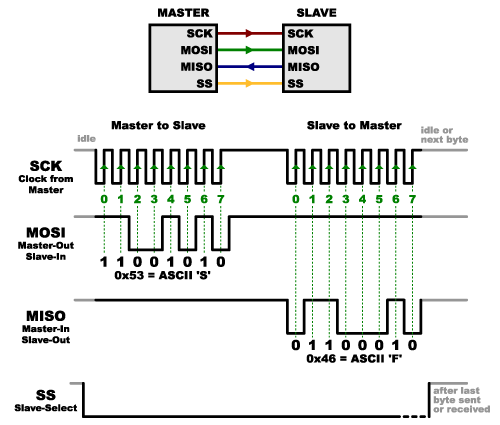
\includegraphics[width=0.7\textwidth]{spi-timing-2.png}
	\caption{Grafico de comunicacion SPI}
\end{figure}

\subsubsection{Ventajas}
Segun Wikipedia\cite{wikipedia_spi}:
\begin{itemize}
	\item Comunicación Full Duplex
	\item Mayor velocidad de transmisión que con I²C o SMBus
	\item Protocolo flexible en que se puede tener un control absoluto sobre los bits transmitidos
	\item No está limitado a la transferencia de bloques de 8 bits
	\item Elección del tamaño de la trama de bits, de su significado y propósito
	\item Su implementación en hardware es extremadamente simple
	\item Consume menos energía que I²C o que SMBus debido que posee menos circuitos (incluyendo las resistencias pull-up) y estos son más simples
	\item No es necesario arbitraje o mecanismo de respuesta ante fallos
	\item Los dispositivos clientes usan el reloj que envía el servidor, no necesitan por tanto su propio reloj
	\item No es obligatorio implementar un transceptor (emisor y receptor), un dispositivo conectado puede configurarse para que solo envíe, sólo reciba o ambas cosas a la vez
	\item Usa mucho menos terminales en cada chip/conector que una interfaz paralelo equivalente
	\item Como mucho una única señal específica para cada cliente (señal SS), las demás señales pueden ser compartidas
\end{itemize}

\subsubsection{Desventajas}
\begin{itemize}
	\item Consume más pines de cada chip que I²C, incluso en la variante de 3 hilos
	\item El direccionamiento se hace mediante líneas específicas (señalización fuera de banda) a diferencia de lo que ocurre en I²C que se selecciona cada chip mediante una dirección de 7 bits que se envía por las mismas líneas del bus
	\item No hay control de flujo por hardware
	\item No hay señal de asentimiento. El servidor podría estar enviando información sin que estuviese conectado ningún cliente y no se daría cuenta de nada
	\item No permite fácilmente tener varios servidores conectados al bus
	\item Sólo funciona en las distancias cortas a diferencia de, por ejemplo, RS-232, RS-485, o Bus CAN
\end{itemize}
\clearpage

\subsection{Protocolo I2C}
\begin{wrapfigure}{r}{0in}
	\centering
	
\includegraphics[width= 1.5in, keepaspectratio]{I2C_logo.png}
	\caption{Logo de I2C}
\end{wrapfigure}
El protocolo I2C es un protocolo de comunicacion entre circuitos integrados,
en el cual se definen dispositivos a funcionar como maestros o \emph{master},
y dispositivos a funcionar como esclavos o \emph{slave}. \\
Lo que se hace es establecer comunicacion entre los dispositivos usando dos lineas:
\begin{itemize}
	\item SCL (\textbf{S}erial \textbf{CL}ock):
	      Es la linea que transmite la señal de sincronía.\\
	      Eléctricamente se trata de una señal a colector o drenador abierto.
	      En un dispositivo esclavo se trata de una entrada,
	      mientras que en un dispositivo maestro es una salida.\\
	      El dispositivo maestro genera la señal de sincronía, necesaria para
	      mantener la comunicación entre los dispositivos.
	\item SDA (\textbf{S}erial \textbf{DA}ta):
	      Es la linea que transmite los datos de forma semi-bidireccional.\\
	      Eléctricamente se trata de una señal a colector o drenador abierto.
	      Es gobernada por el emisor, sea éste un maestro o un esclavo.\\
	      Sobre esta linea se montan los datos a transmitir entre los dispositivos.
\end{itemize}

\end{document}